\documentclass{standalone}

%----------------------------------------------------------------------------------------------%
%                                 Packages and basic declarations
%----------------------------------------------------------------------------------------------%

\usepackage[utf8]{inputenc}
\usepackage{pgfplots}
\usepackage{tikz}


%----------------------------------------------------------------------------------------------%
%----------------------------------------------------------------------------------------------%
%                                            DOCUMENT STARTS
%----------------------------------------------------------------------------------------------%
%----------------------------------------------------------------------------------------------%

\begin{document}


%Tikz picture starts%

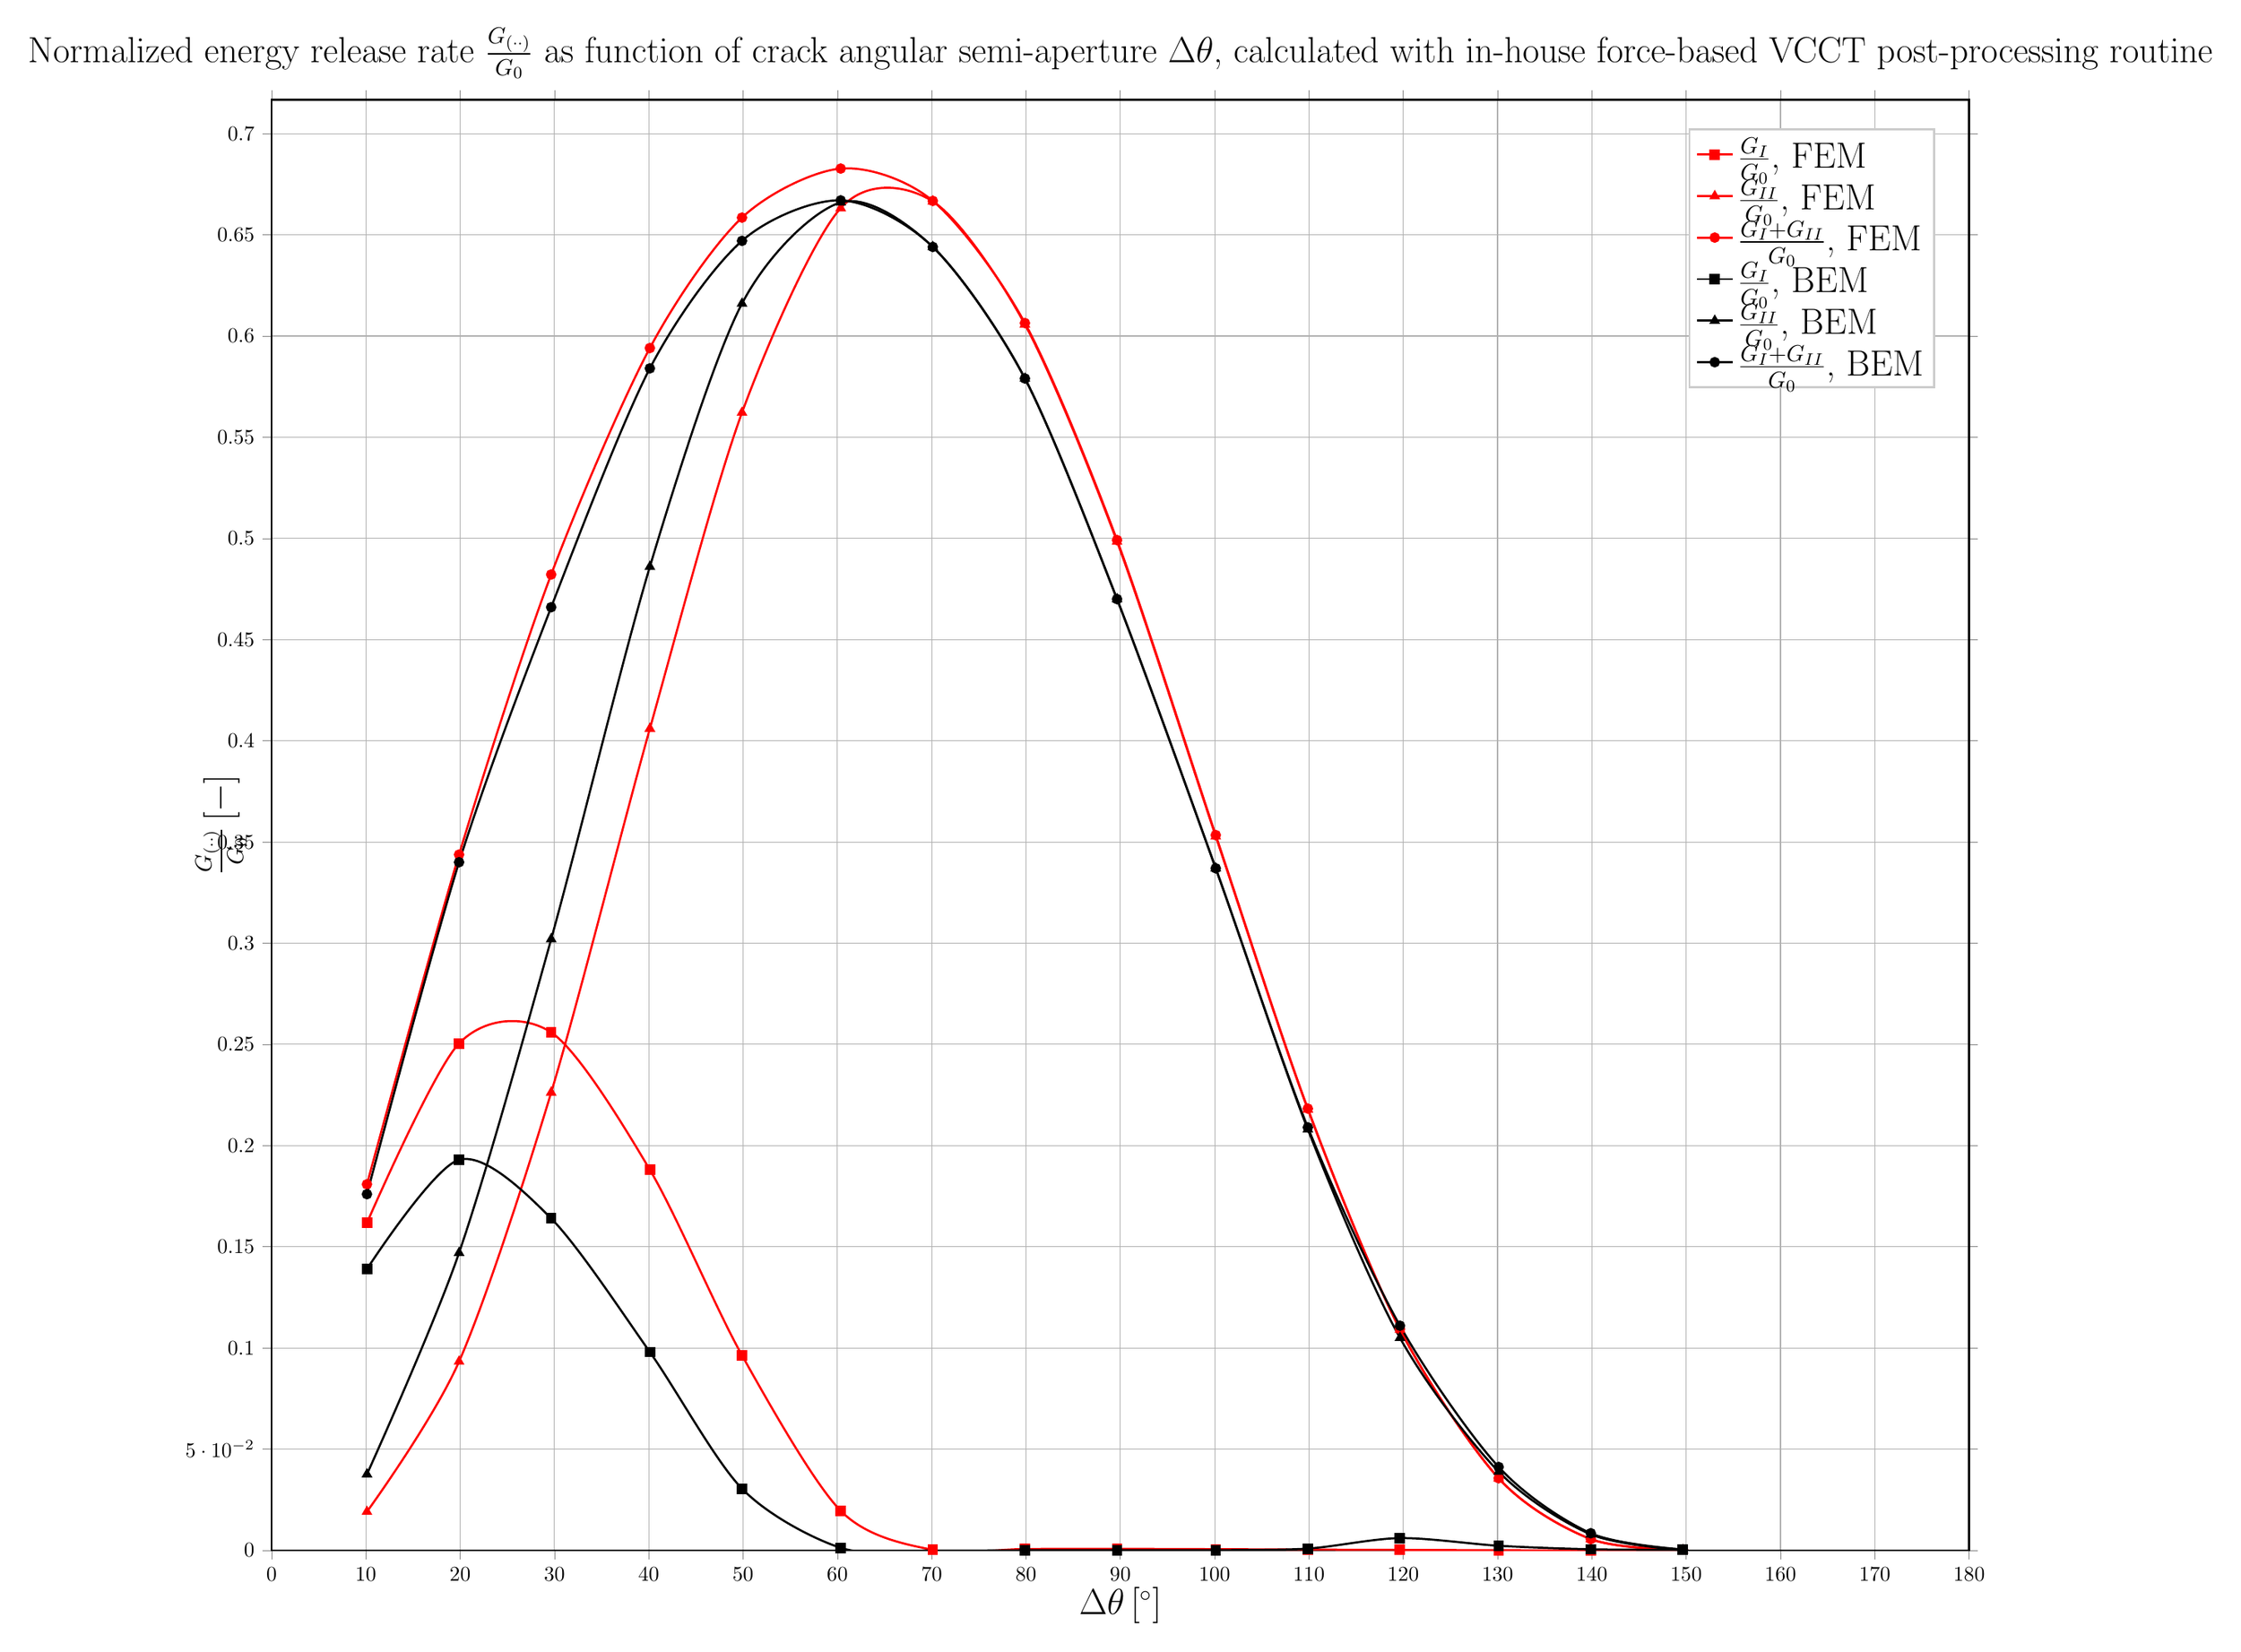
\begin{tikzpicture}

%Tikz axis starts%

\begin{axis}[width=30cm,
title={Normalized energy release rate $\frac{G_{\left(\cdot\cdot\right)}}{G_{0}}$ as function of crack angular semi-aperture  $\Delta\theta$, calculated with in-house force-based VCCT post-processing routine},
title style={font=\fontsize{16}{8}\selectfont},
xlabel style={at={(axis description cs:0.5,-0.02)},anchor=north,font=\fontsize{16}{8}\selectfont},
ylabel style={at={(axis description cs:-0.01,.5)},anchor=south,font=\fontsize{16}{8}\selectfont},
xlabel={$\Delta\theta\left[^{\circ}\right]$},ylabel={$\frac{G_{\left(\cdot\cdot\right)}}{G_{0}}\left[-\right]$},
xmin=0.0,
xmax=180.0,
ymin=0.0,
ymax=0.716856184339,
tick align=outside,
tick label style={font=\normalsize},
xtick={0.0,10.0,20.0,30.0,40.0,50.0,60.0,70.0,80.0,90.0,100.0,110.0,120.0,130.0,140.0,150.0,160.0,170.0,180.0},
xmajorgrids,
x grid style={lightgray!92.026143790849673!black},
ymajorgrids,
y grid style={lightgray!92.026143790849673!black},
line width=0.35mm,
legend style={draw=white!80.0!black,font=\fontsize{16}{12}\selectfont},
legend entries={{$\frac{G_{I}}{G_{0}}$, FEM},{$\frac{G_{II}}{G_{0}}$, FEM},{$\frac{G_{I}+G_{II}}{G_{0}}$, FEM},{$\frac{G_{I}}{G_{0}}$, BEM},{$\frac{G_{II}}{G_{0}}$, BEM},{$\frac{G_{I}+G_{II}}{G_{0}}$, BEM}},
legend cell align={left}
]

\addplot[red,smooth,mark=square*]
table{
10.1165133448 0.161791260912
19.8836864193 0.250481963169
29.6513572437 0.255928474844
40.1161769391 0.188043616057
49.8838221503 0.0963771099078
60.3486418456 0.0195696822849
70.1163109626 0.000244483311321
79.8834883059 0.000680342228526
89.651164253 0.000758800354777
100.116516703 0.000600349395434
109.883687216 0.000389041056218
119.651363163 0.000247953959058
130.116182859 8.8611855244e-05
139.883817825 1.44831441088e-05
149.651466451 0.000289733197074
};

\addplot[red,smooth,mark=triangle*]
table{
10.1165133448 0.0190905672935
19.8836864193 0.093291527899
29.6513572437 0.226223106143
40.1161769391 0.406001744225
49.8838221503 0.56211362784
60.3486418456 0.663150493277
70.1163109626 0.666495212627
79.8834883059 0.605704911159
89.651164253 0.498407457823
100.116516703 0.352810675218
109.883687216 0.217883068048
119.651363163 0.109090753588
130.116182859 0.0355691277155
139.883817825 0.00557389800812
149.651466451 7.92869012139e-05
};

\addplot[red,smooth,mark=*]
table{
10.1165133448 0.180881828206
19.8836864193 0.343773491068
29.6513572437 0.482151580987
40.1161769391 0.594045360283
49.8838221503 0.658490737747
60.3486418456 0.682720175561
70.1163109626 0.666739695938
79.8834883059 0.606385253387
89.651164253 0.499166258177
100.116516703 0.353411024613
109.883687216 0.218272109104
119.651363163 0.109338707547
130.116182859 0.0356577395707
139.883817825 0.00558838115223
149.651466451 0.000369020098288
};

\addplot[black,smooth,mark=square*]
table{
10.1165133448 0.139
19.8836864193 0.193
29.6513572437 0.164
40.1161769391 0.098
49.8838221503 0.0305
60.3486418456 0.00127
70.1163109626 -4.79e-05
79.8834883059 6.85e-05
89.651164253 0.000112
100.116516703 0.000112
109.883687216 0.000895
119.651363163 0.00607
130.116182859 0.00229
139.883817825 0.000552
149.651466451 0.000306
};

\addplot[black,smooth,mark=triangle*]
table{
10.1165133448 0.0376
19.8836864193 0.147
29.6513572437 0.302
40.1161769391 0.486
49.8838221503 0.616
60.3486418456 0.666
70.1163109626 0.644
79.8834883059 0.579
89.651164253 0.47
100.116516703 0.337
109.883687216 0.208
119.651363163 0.105
130.116182859 0.0389
139.883817825 0.00792
149.651466451 0.000165
};

\addplot[black,smooth,mark=*]
table{
10.1165133448 0.176
19.8836864193 0.34
29.6513572437 0.466
40.1161769391 0.584
49.8838221503 0.647
60.3486418456 0.667
70.1163109626 0.644
79.8834883059 0.579
89.651164253 0.47
100.116516703 0.337
109.883687216 0.209
119.651363163 0.111
130.116182859 0.0412
139.883817825 0.00847
149.651466451 0.000471
};

\end{axis}
%Tikz axis ends%


\end{tikzpicture}
%Tikz picture ends%


\end{document}

%----------------------------------------------------------------------------------------------%
%----------------------------------------------------------------------------------------------%
%                                            DOCUMENT ENDS
%----------------------------------------------------------------------------------------------%
%----------------------------------------------------------------------------------------------%

